\chapter{Methodology}\label{ch:B}
\section{Agile}\label{agile}
\begin{figure}[ht]\label{fig:agile}
  \centering
  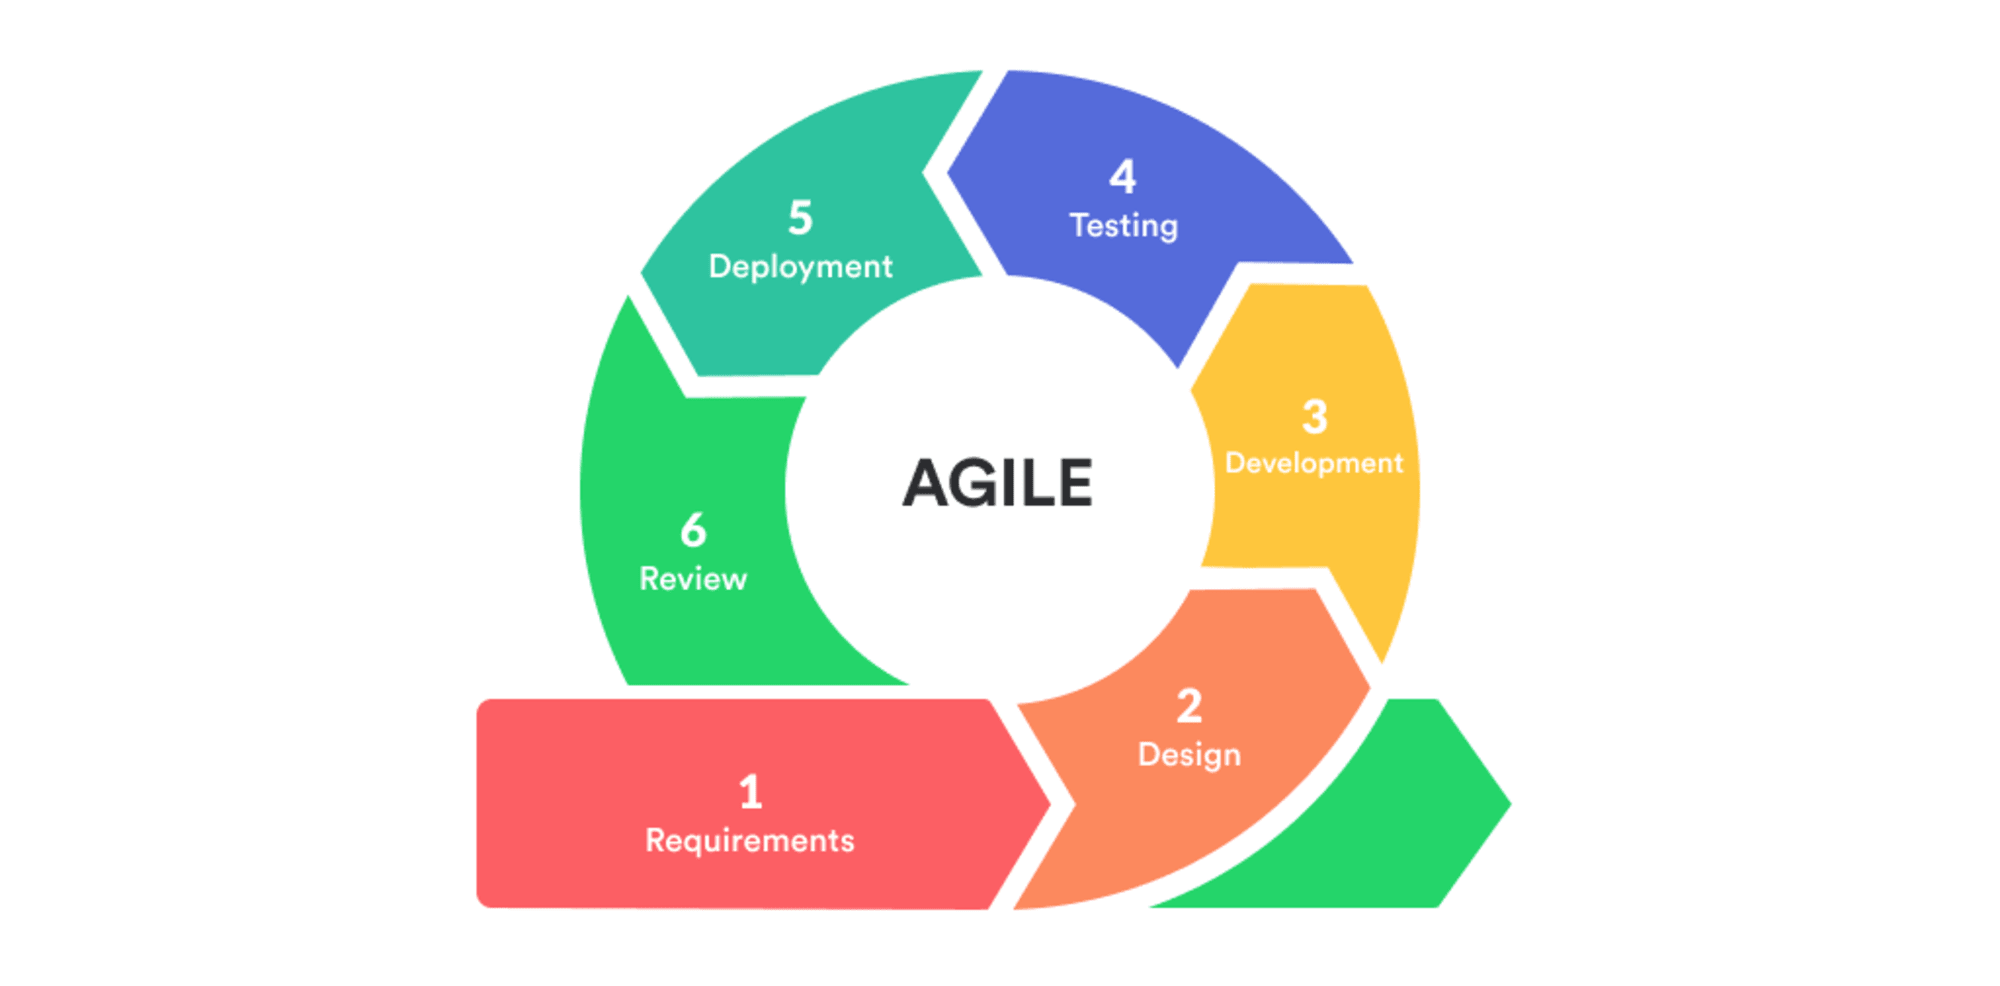
\includegraphics[width=0.8\linewidth]{figures/agile.png}
  \caption{Agile methodology.}
\end{figure}
\vspace{0.5cm}

In our project, we focus on successful implementation from the moment of initiation to the MVP (Minimum Viable Product) \cite{mvp} of the product, we focus on the philosophy of flexible project management, an agile methodology \cite{agile} that promotes better adaptation to various changes during the project. 
Let us figure out a little about agile \cite{agile}. This is a philosophy of flexible project management philosophy that promotes rapid adaptation to changes, as well as a modern approach in which the team works together with the customer to determine the needs of the project. \textbf{There are also 4 principles of the Agile Manifesto:} \cite{agilemanifesto}:

\begin{enumerate}
\item People and interaction are \textbf{more important} than processes and tools.
\item A working product is \textbf{more important} than comprehensive documentation.
\item Cooperation with the client is \textbf{more important} than agreeing on the terms of the contract.
\item Being ready for change is \textbf{more important} than following the original plan. 
\end{enumerate}

At the beginning of the our project, we conducted some kind of brainstorming, then highlighted this project idea, then we were engaged in creating project documentation, and this is the project charter plan \cite{projectcharter}, Gantt chart \cite{gantChart}, communication plan \cite{communicationplant}, split our work into 15 weeks in we call as sprints, in each 1 week for to do tasks, used the SCRUM \cite{scrumguide} framework, project execution plan \cite{executionplan}, RACI Chart \cite{racichart}, who is responsible for what - SWOT analysis chart \cite{swotanalyse} what are the strengths and the weaknesses of the team, the risks \cite{risksanalyse}, and the analysis of stakeholders. We also called once every 3-4 weeks by discord \cite{discord} and telegram \cite{telegram} to support the plan and discuss the project. Also, during the project, we created a product backlog in JIRA using the KANBAN board \cite{jira} and worked through this application. After one sprint, we conducted a task test to identify bugs also we played in scrum poker for identify for speed for each tasks in story point which means that how many days to do task need to.

\section{Scrum + Kanban}\label{scrmkan}
\begin{figure}[ht]\label{fig:kanbanboard}
  \centering
  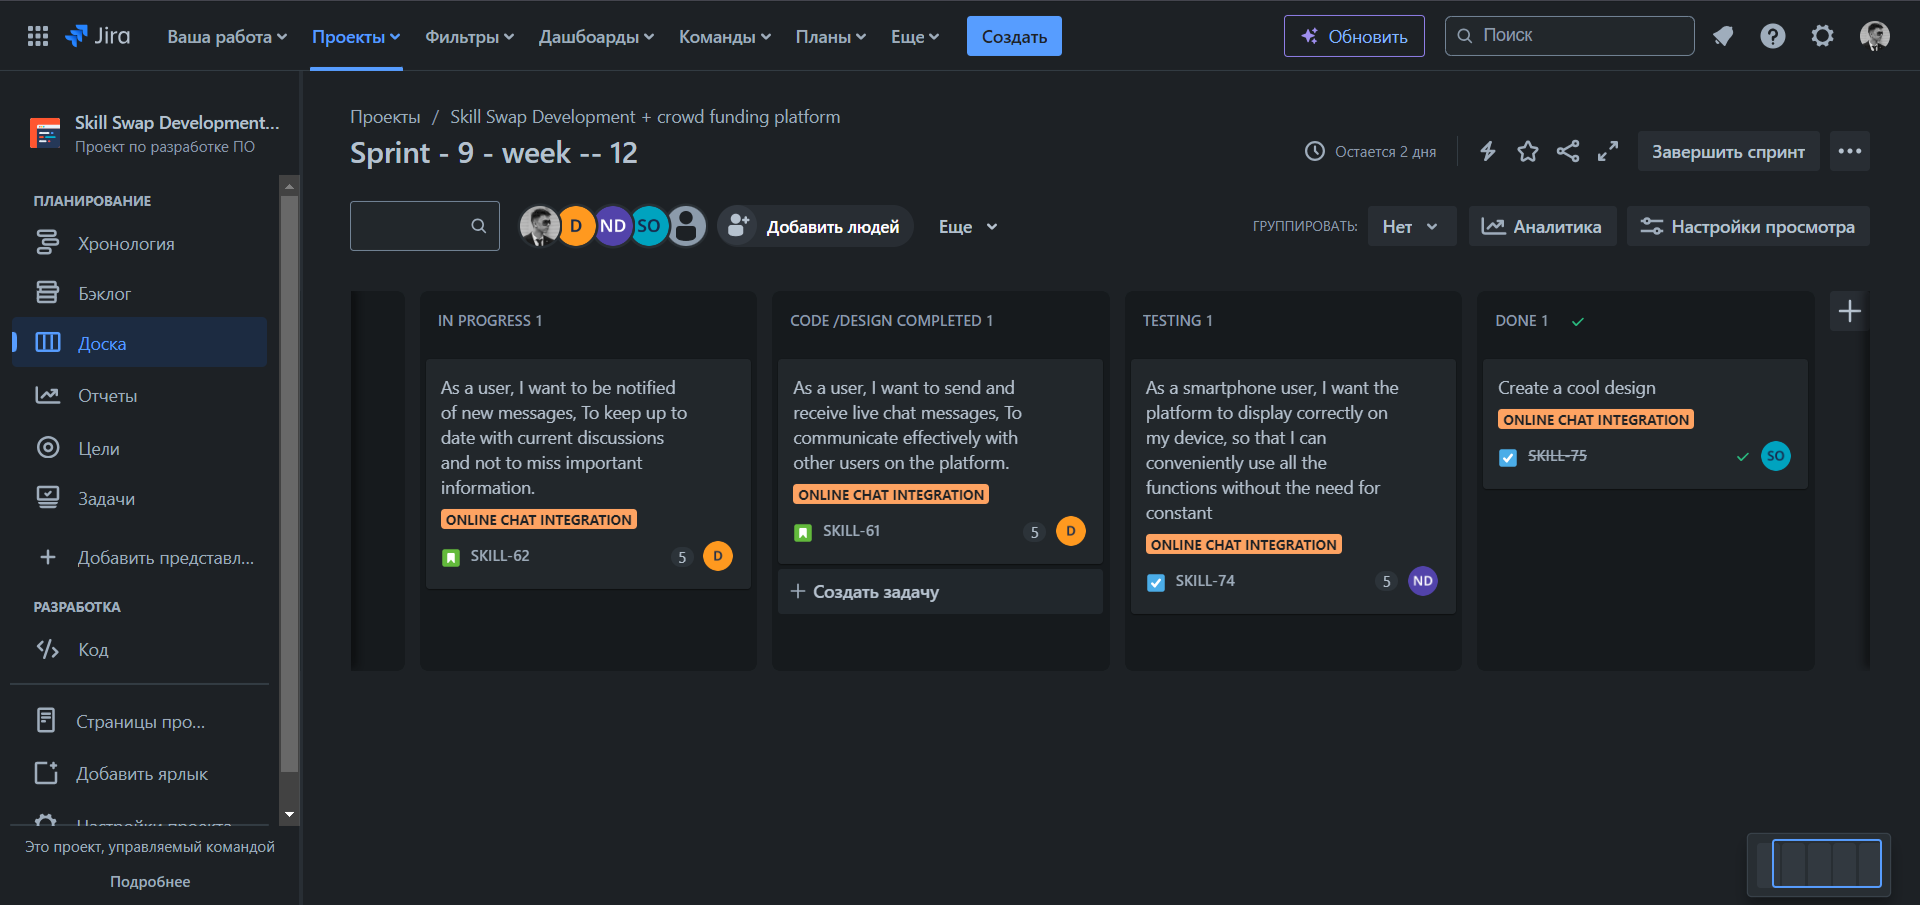
\includegraphics[width=0.8\linewidth]{figures/Kanban board.png}
  \caption{Scrum sprint + Kanban board.}
\end{figure}

Agile philosophy \cite{agile} has its own frameworks, the most popular of them is Scrum + Kanban \cite{jira}. We worked on framework which name is scrum, that is, we determined what values the team had and also determined the team's responsibilities. In this case, our team turned into a cross-functional one. Let's take a little look at what a scrum is \cite{scrumguide}. Scrum is a lightweight framework that helps people, teams, and organizations create value through adaptive solutions and to solve complex problems. \textit{Components:} An iterative approach with a team of up to 10 people working in sprints (1 (2) - 4 weeks). Scrum clearly defines values, roles, and procedures that will help employees focus on repetitive work and its continuous improvement.
\newpage
Team roles in the scrum team \cite{scrumguide}:

\begin{itemize}
    \item \textbf{Scrum Master} - ensures compliance with processes in our case this is  (Project Manager).
    \item \textbf{Product owner} - defines the requirements for the product (Our diploma instructor).
    \item \textbf{Developers} - implement the product (team). 
\end{itemize}

Now to kanban \cite{kanban}, this is a visualization method that gives additional motivation to accomplish the goal of kanban itself, the board is divided into: 

\begin{itemize}
    \item \textbf{To Do} - what should we to do with our project. For example: As a user, I want to easily navigate the main page, so that i can understand the purpose and features of the platform.
    \item \textbf{In process} - what currently develop 
    \item \textbf{Testing} - if task complete by full - stack developer then Quality Assurance test their work.
    \item \textbf{Done} - after test if all is well then this work is complete.
    
\end{itemize}

\section{Business analytics our team}\label{bussanl}
On the basis of the preliminary analysis, we have started the project implementation process. To do this, we have distributed roles and responsibilities in the following order for be a cross-functional team:

\begin{itemize}
    \item Ossipov Alexandr - 200103001@stu.sdu.edu.kz, Team lead Project Manager. 
    \item Daulet Lepessov  - 200103213@stu.sdu.edu.kz, Full-Stack - developer. 
    \item Nurlan Darzhanov - 200103481@stu.sdu.edu.kz, IOS - developer. 
    \item Saya Oryskhan  - 200103459@stu.sdu.edu.kz, UX/UI + Quality Assurance.  
\end{itemize}

Now let's take a closer look at what each team member was doing. Let us start with the \textbf{first member} of the team with the project manager and team leader, \textit{Alexandr Ossipov}. In the course of this work, a lot was done: We divided the project into 4 parts, and this is the moment.

\begin{enumerate}
    \item \textbf{Initiations} - Brainstorm read diploma in structure. 
    \item \textbf{Planning} - Create plan for this project deadlines and etc. 
    \item \textbf{Execution and documentation} - Execute project by documentation. 
    \item \textbf{Closing the project} - writing a thesis and deploying our product.
\end{enumerate}

 Further, during this project, he organized online discord \cite{discord} and telegram meetings \cite{telegram}, monitored the quality of sprints and deadlines, motivated each team member for the successful implementation of various tasks, did some brainstorming prototyping the application and website together with the team at the initial stage of the project. We also created various documentation: the project charter \cite{projectcharter}, the project execution plan \cite{executionplan}, and so on. All links in the following are attached in references part. 
\vspace{0.5cm}
\par
\textbf{The second member} of the team is our full-stack developer \textit{Daulet Lepessov}. During this project, he was a key member of the team since our main application is a website. During the execution, he did a lot of work, wrote more than one thousand lines of code for the excellent operation of the application, followed strict deadlines, used the laravel \cite{laravel} framework with the PHP programming language, this was the \nameref{back} part. He also did \nameref{front} work, wrote a visual of the site, and used node for design, using frameworks: REACT.JS \cite{react} + HTML + CSS + JS\cite{htmlcssjs} + bootstrap\cite{boostrap} + jQuery\cite{jquery}.
\vspace{0.5cm}
\par
Our \textbf{third team member} is also a key one, \textit{Nurlan Darzhanov}, he is our \nameref{ios} developer, he made an application for iPhones using the Swift programming language \cite{swift}. 
\vspace{0.5cm}
\par
And finally, our \textbf{fourth team member} is \textit{Saya Oryskhan}, too, she was our \nameref{des} and \nameref{qa}, she made the coolest design using UX/UI \cite{design} on that, for a web application and a phone application, all screenshots will be attached below in references part and at the end of each sprint she tested the tasks that were on each week to help developers make the product better.